\section*{Synthesizing Measures of State Preference}

The approach that we introduce here to measure state preference similarity starts by assuming that both UN voting and alliance relationships are sources of information on how states relate to one another on the international stage. By accounting for the multiple layers upon which states interact with one another we can synthesize a better measure of preference similarity than if we relied on any one measure alone. The idea of using multiple metrics to get a better handle on preferences is not new, in fact, Signorino and Ritter suggested it in introducing S-scores, which were designed to allow for aggregation of similarity on multiple dimensions (such as alliances and UN voting). The downside of this extant approach, however, is that it does not account for structural patterns that we often see in relational data.

Relational data is composed of observations between pairs of actors, or dyads. For both alliance relationships and UN voting, we are able to observe how the actors in the international system interact with one another across time. This system of interactions taken in its totality defines a network, and within these types of structures a bevy of research has shown that we need methods that go beyond assuming that interactions are taking place between just two actors in a vacuum \citep{wasserman:faust:1994,snijders:nowicki:1997,minhas:etal:2019}. As such we reformulate the problem of determining state preferences in terms of a network analysis. The goal of our approach is summarized in Figure~\ref{fig:tensViz}. In the top row, we represent UN voting and alliance patterns at time $t$ as a pair of adjacency matrices that form an evolving multiplex network.\footnote{The approach that we describe here can be generalized to a multiplex with more than two dimensions.} Our goal is to extract a lower dimensional representation of this system, such that the output is a series of $n \times n$ matrices, where $n$ represents the number of actors and in which the cross-sections denote our estimates of the preference similarities between countries.

\begin{figure}[ht]
	\centering
	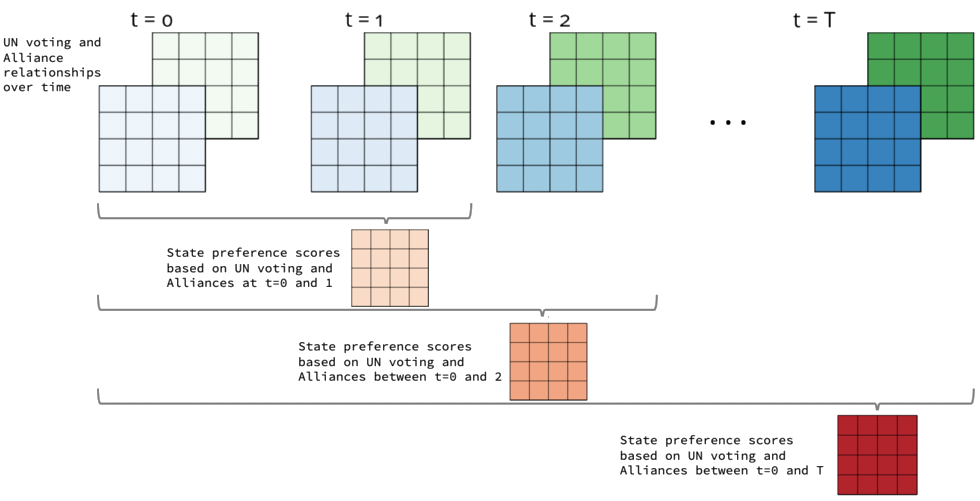
\includegraphics[width=1\textwidth]{tensor_viz.png}
	\caption{The green and blue colors represent different relational measures and darker shading indicates later time periods. Our goal is to reduce the patterns found across those layers of relationships into a single measure.}
	\label{fig:tensViz}
\end{figure}

We generate these estimates through a multilinear tensor regression model that combines information across networks and time to measure how dependent the actions of a particular state are on another \citep{hoff:2015,minhas:etal:2016}. By incorporating information from multiple measures through a network perspective, we show that our approach improves on alternative measurements of state preference when it comes to predicting and explaining interstate conflict.

\subsection*{Multilinear Tensor Regression}

Our goal here is to measure a concept that is not directly observable. This is a problem that is very familiar in political science and a number of techniques based on measurement models have been developed to study political ideology \citep{martin:quinn:2002,konig:etal:2013}, human rights abuses \citep{fariss:2014}, and judicial independence \citep{linzer:staton:2015}. Obviously, the ideal points measure developed by \citet{bailey:etal:2015} also follows in this growing practice of extracting unobserved information via a spatial weighting scheme. Here we build on this general goal by developing a measurement of how a state relates to other states in a network context. Substantively, this goal is no different than how others have sought to find simpler representations of legislators and bills \citep{poole:rosenthal:1985,clinton:etal:2004}, but the key difference from shifting to the network is the recognition that we can better understand the relations between a pair of states by understanding how they relate to others in the international system.

We represent relational data that is longitudinal as an array $\bl Y = \{\bl Y_t : t = 1, \ldots T\}$, with each $\bl Y_t$ representing the actions between countries in a given year $t$. A cross-sectional entry such as $y_{i,j,v,t}$ from $\bl Y$ denotes an interaction that occurred between actors $i$ and $j$ at time $t$ across variable $v$. These series of matrices can be assembled in a tensor, $\bl Y$, which we use to represent actors interacting over time across multiple measures. Specifically, $\bl Y$ will have dimensions $n \times n \times p \times T$, where $n$ corresponds to the number of countries, $p$ to the number of variables (i.e., relational measures), and $T$ to the number of time periods.

The information contained in this set of matrices can also be represented as a vector, where $(\mathbf y_t)$ represents a time series of vectors representing the dyadic interactions across multiple variables for $n$ countries through the period $t = 1, \ldots, T$. Transforming the data in this way enables us to think of what we are modeling in an explicitly time series context, where the evolution of multiple series is a function of their past behavior. Modeling such processes can often be accomplished using a vector autoregression (VAR) framework:

\begin{eqnarray}
	\bl y_t &=& { \Theta \bl y_{t-1} +\bl e_t}\\
	E[\bl e_t] &=& 0 \\
	E[\bl e_t \bl e^T_s] &=& \begin{cases}   \Sigma &\mbox{if } t=s, \\ 0 &\mbox{otherwise}\end{cases}
\end{eqnarray}

However, given the data requirements of estimating $\Theta$,\footnote{$\Theta$ has $n^4$ entries.} \citet{hoff:2015} employs a bilinear regression model such that the regression matrix is given by $ \Theta = \bl B \otimes \bl A$.\footnote{$\otimes$ is the Kronecker product.} As a result, we obtain the following basic specification: $\bl Y_t = \bl A \bl Y_{t-1}\bl B^T$. An alternative approach to this tensor decomposition could have involved the usage of a network latent variable model scheme. The key difference between those models and this tensor approach is that in the former we are projecting the relations between actors onto lower a dimensional space, where similarity in orientation indicates that actors are more likely to have similar dependence patterns. In the context of this model, $\bl A$ and $\bl B$ are $n \times n$ matrices of regressions coefficients, where each cross-sectional entry measures the level of dependence between the sending relationships of a particular actor and  $B$ the receiving relationships.

The tensor regression problem can also be written somewhat more simply in tensor form, where it is clearer that we are essentially regressing the relational tensor $\bl Y_t$ from time $t$ on the tensor $\bl Y_{t-1}$ from time $t-1$:

\begin{equation}
	\bl Y = \bl Y_{t-1} \boldsymbol{\times} \{ \bl A, \bl B \} + \bl E ,
	\label{eqn:mltr}
\end{equation}

``$\boldsymbol{\times}$'' is a multilinear operator known as the ``Tucker product''. The Tucker product is used for higher-order singular value decomposition (SVD), the same way that matrix multiplication is used for matrix SVD \citep{kolda:bader:2009}. To illustrate how the Tucker product is calculated, say that we want to get the following expression: $\bl Y = \bl Y_{t-1} \boldsymbol{\times} \{ \bl A, \bl B\},$ where $\bl Y$ has dimensions $n_{1} \times n_{2} \times n_{3}$ and $\bl Y_{t-1}$ has dimensions $m_{1} \times m_{2} \times m_{3}$. The first step involves reshaping $\bl Y_{t-1}$ so that it is a matrix with  dimensions $m_{1} \times (m_{2} \times m_{3})$, then we multiply on the left by $\bl A$, next we reshape the result to an $n_{1} \times (m_{2} \times m_{3})$ matrix.\footnote{Further details on this operator can be found in \citet{kolda:2006}.} This procedure would be applied iteratively among the remaining dimensions. We estimate this via Gibbs sampling using the procedure discussed in Hoff (2015). In modeling the error distribution we utilize an array normal model for the error distribution, which is a multivariate normal model with a Kronecker structred covariance matrix. \citet{akdemir:gupta:2011} and \citet{hoff:2011a} show that this provides a flexible, reduced parameter covariance model that still accounts for the tensor structure of the data.\footnote{In our application, we say that $\bl E$ has a mean-zero array normal distribution, $\bl E \sim N(0, \Sigma_{\bl A}, \Sigma_{\bl B})$.}

The key parameters that we seek to estimate from this model are $\bl A$ and $\bl B$.\footnote{Note that for a given ordered pair of nodes $(i_{1},i_{2})$, $E[y_{i_{1},i_{2},t} | \bl Y_{t-1}] = \sum_{j_{1}} \sum_{j_{2}} a_{i_{1},j_{1}} b_{i_{2},j_{2}} y_{j_{1},j_{2},t-1}$. Where $a_{i_{1},j_{1}}$ describes how actions by $i_{1}$ are influenced by the previous actions of $j_{1}$, and $b_{i_{2},j_{2}}$ describes how actions received by $i_{2}$ are influenced by previous actions towards $j_{2}$.} These contain $n \times n$ regression coefficients and represent how previous actions along any of the $v$ parameters affect future interactions. The $ij$ coefficient in $\bl A$ measures the effect of an interaction from actor $j$ to actor $k$ along any of the $v$ parameters on the likelihood of an interaction from $i$ to $k$ in the next time period. Specifically, $a_{i,i'}$ capture how previous actions of $i'$ affect $i$ and $b_{j,j'}$ shows how actions that target $j$ are influenced by prior actions toward $j'$. If $a_{i,i'}$ is positive, this gives us a measure of how likely $i$ is to send an event to a third party $k$ given that $i'$ has already sent an event to $k$. More concretely, if we imagine that the event is alliance formation, then a positive $a_{i,i'}$ would indicate that $i$ and $i'$ are more likely to initiate alliances with the same third country. If $b_{j,j'}$ is positive on the other hand, this gives us a measure of how likely $j$ is to receive an alliance request from a third party $k$ given that $j'$ has already received that event from $k$. Taken together, A and B measure how similar each of the actors behave towards third parties.

This maps well to the field's understanding of state preference similarity. If states have similar preferences, they will react similarly to a common situation or stimuli. If two states have positive (negative) values for $\bl A$ and $\bl B$, we will see convergence (divergence) in their behavior to a set of resolutions at the United Nations or the opportunity to ally with a particular state; we infer from this that they have (dis)similar preferences.
